\section{Design}

FlashR provides parallelized matrix operations in R for machine learning and
statistics. It scales matrix operations beyond memory capacity by utilizing
fast I/O devices, such as solid-state drives (SSDs), in a non-uniform memory
access (NUMA) machine. Figure \ref{fig:arch} shows the architecture of FlashR.
FlashR supports a small number of classes of generalized operations (GenOps)
and uses GenOps to implement many matrix operations in the R base package
to provide users a familiar programming interface. The GenOps simplify
the implementation and improve expressiveness of the framework. The optimizer
aggressively merges operations to reduce data movement in the memory hierarchy.
FlashR stores matrices on SSDs through SAFS \cite{safs}, a user-space filesystem
for SSD arrays, to fully utilize high I/O throughput of SSDs.

FlashR supports both sparse matrices and dense matrices. For large sparse matrices,
FlashR integrates with the work \cite{SEM_SpMM} that stores sparse matrices
in a compact format on SSDs and performs sparse matrix multiplication
in semi-external memory, i.e., keeping the sparse matrix on SSDs and
the dense matrix or part of the dense matrix in memory.

\begin{figure}
\centering
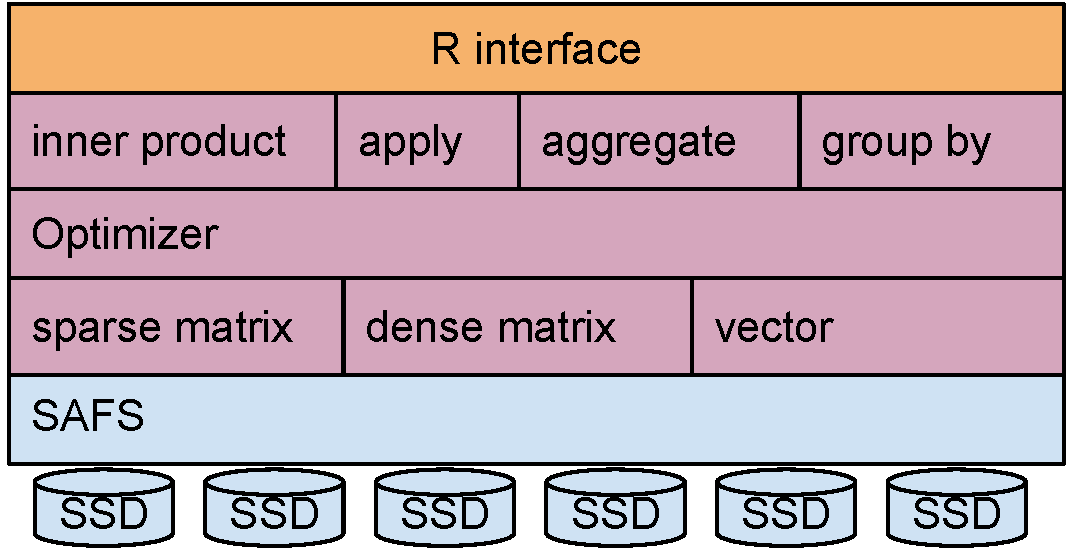
\includegraphics[scale=0.3]{FlashMatrix_figs/architecture.pdf}
\vspace{-5pt}
\caption{The architecture of FlashR.}
\label{fig:arch}
\vspace{-10pt}
\end{figure}

\subsection{Dense matrices}
FlashR optimizes for dense matrices that are rectangular---with
a longer and shorter dimension---because of their frequent occurrence
in machine learning and statistics. Dense matrices can be stored
physically in memory or on SSDs or represented virtually by a sequence of
computations.

\subsubsection{Tall-and-skinny (TAS) matrices}
A data matrix may contain a large number of samples with a few features
(tall-and-skinny),
or a large number of features with a few samples (wide-and-short).
We use similar strategies to optimize wide-and-short matrices. FlashR
supports both row-major and column-major layouts (Figure \ref{fig:den_mat}(a)
and (b)), which allows FlashR to transpose matrices without a copy.
We store vectors as a one-column TAS matrix.

\begin{figure}
	\centering
	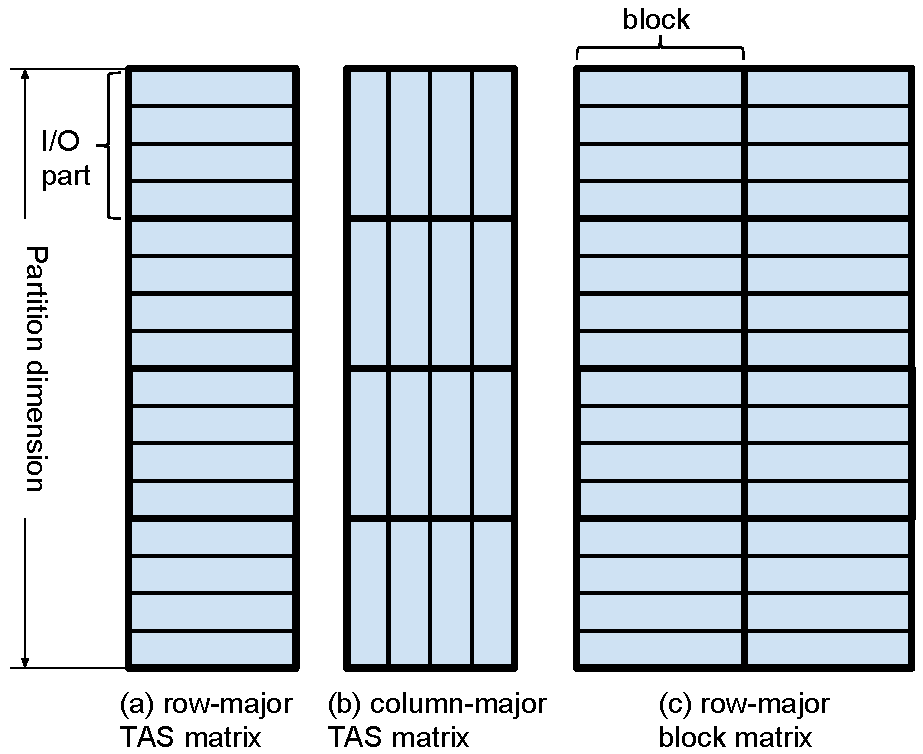
\includegraphics[scale=0.5]{FlashMatrix_figs/dense_matrix2.pdf}
	\vspace{-5pt}
	\caption{The format of a tall dense matrix.}
	\label{fig:den_mat}
  \vspace{-12pt}
\end{figure}

A TAS matrix is partitioned physically into I/O-partitions (Figure
\ref{fig:den_mat}). We refer to the dimension that is partitioned as
the \textit{partition dimension}. All elements in an I/O-partition are stored
contiguously regardless of the data layout in the matrix. All I/O-partitions
have the same number of rows regardless of the number of columns in a TAS
matrix. The number of rows in an I/O-partition is always $2^i$, where
$i \in \mathbb{N}$. This produces column-major TAS
matrices whose data are well aligned in memory to encourage CPU vectorization.

When a TAS matrix is stored in memory, FlashR stores its I/O partitions in
fixed-size memory chunks (e.g., 64MB) across NUMA nodes.
I/O partitions from different matrices may have different sizes. By storing
I/O partitions in fixed-size memory chunks shared among all in-memory matrices,
FlashR can easily recycle memory chunks to reduce memory allocation overhead.
%Because all in-memory
%matrices are distributed across NUMA nodes in the same fashion,
%FlashR schedules threads to perform computation on I/O partitions
%in the memory close to the processors to increase the memory bandwidth.

When a TAS matrix is stored on SSDs, it is stored as a SAFS file \cite{safs}.
For such a matrix, an I/O partition is accessed in a single I/O request.
We rely on SAFS to map the data of a matrix evenly across SSDs. SAFS allows
applications to specify the data mapping strategies. By default, FlashR uses
a hash function to map data to SSDs to fully utilize the bandwidth of all SSDs
even if we access only a subset of columns from a TAS matrix.

\subsubsection{Block matrices} \label{sec:block_mat}
FlashR stores a tall matrix as a \textit{block matrix}
(Figure \ref{fig:den_mat}(c)) comprised of TAS blocks with $32$ columns each,
except the last block. Each block is stored as a separate TAS matrix.
We decompose a matrix operation
on a block matrix into operations on individual TAS matrices to take advantage
of the optimizations on TAS matrices and reduce data movement.
Coupled with the I/O partitioning on TAS matrices, this strategy enables
2D-partitioning on a dense matrix and each partition fits in main memory.

%\dz{Should we explain GenOps on block matrices in more details?}

%\subsection{Sparse matrices}
%FlashR supports sparse matrices and optimizes sparse matrices of different
%shapes differently.
%For large sparse matrices that arise from graphs (e.g., social networks
%and Web graphs), which have a large number of rows and columns, FlashR integrates
%with our prior work \cite{SEM_SpMM} that stores sparse matrices
%in a compact format on SSDs and performs sparse matrix multiplication
%in semi-external memory, i.e., we keep the sparse matrix on SSDs and
%the dense matrix or part of the dense matrix in memory.
%Because many graph algorithms can be formulated with sparse matrix multiplication
%\cite{linear_algebra}, we can express these algorithms in FlashR. In contrast,
%for sparse matrices with many rows and few columns or with many columns
%and few rows, FlashR stores the sparse matrices with the coordinate format
%(COO). These sparse matrices can be used in sparse random projection
%\cite{sparse_proj} or to store categorial values for computation.
%FlashR keeps these sparse matrices in memory.

\subsection{Programming interface} \label{sec:api}

FlashR provides a matrix-oriented functional programming interface built
on Generalized Operations (GenOps). Instead of parallelizing each R matrix 
function individually, FlashR simplifies the implementation by providing
a small set of GenOps and using the GenOps to parallelize R matrix functions.
GenOps (Table \ref{tbl:genops}) take matrices and
some functions as input and output new matrices that represent computation results.
The input function defines computation on individual elements in input matrices,
and, in the current implementation, all of these functions for GenOps are predefined.
GenOps provide a flexible and concise programming interface and, thus,
we focus on optimizing the small set of matrix operations. All of
the GenOps are lazily evaluated to gain efficiency (Section
\ref{sec:lazyeval}).

\begin{table}
\begin{center}
\caption{Generalized operations (GenOps) in FlashR. $A$, $B$ and $C$ are
	matrices, and $c$ is a scalar. $f$ is a user-defined function that
	operates on elements of matrices. $A_{i,j}$ indicates the element
	in row $i$ and column $j$ of matrix $A$.}
\vspace{-10pt}
\footnotesize
\begin{tabular}{|l|l|l|}
\hline
GenOp & Description \\
\hline
$C=sapply(A, f)$ & $C_{i,j}=f(A_{i,j})$ \\
$C=mapply(A, B, f)$ & $C_{i,j}=f(A_{i,j}, B_{i,j})$ \\
\hline
$c=agg(A, f)$ & $c=f(A_{i,j}, c)$, $\forall i, j$ \\
$C=agg.row(A, f)$ & $C_i=f(A_{i,j}, C_i)$, $\forall j$ \\
$C=agg.col(A, f)$ & $C_j=f(A_{i,j}, C_j)$, $\forall i$ \\
\hline
$C=groupby(A, f)$ & $C_{k}=f(A_{i,j}, C_{k})$,\\ & where $A_{i, j}=k$, $\forall i,j$ \\
$C=groupby.row(A, B, f)$ & $C_{k,j}=f(A_{i,j}, C_{k,j})$,\\ & where $B_i=k$, $\forall i$ \\
$C=groupby.col(A, B, f)$ & $C_{i,k}=f(A_{i,j}, C_{i,k})$,\\ & where $B_j=k$, $\forall j$ \\
\hline
$C=inner.prod(A, B, f1, f2)$ & $t=f1(A_{i,k}, B_{k,j})$,
\\ & $C_{i,j}=f2(t, C_{i,j})$, $\forall k$ \\
\hline
$C=cum.row(A, f)$ & $C_{i,j}=f(A_{i,j}, C_{i,j-1})$ \\
$C=cum.col(A, f)$ & $C_{i,j}=f(A_{i,j}, C_{i-1,j})$ \\
\hline
\end{tabular}
\normalsize
\label{tbl:genops}
\vspace{-10pt}
\end{center}
\end{table}

GenOps are classified into four categories that describe different data access
patterns.

\noindent \textbf{Element-wise operations}:
\textit{sapply} is an element-wise unary operation; \textit{mapply}
is an element-wise binary operation.

\noindent \textbf{Aggregation}: \textit{agg} computes aggregation over
all elements in a matrix and outputs a scalar value; \textit{agg.row}
computes over all elements in every row and outputs a vector;
\textit{agg.col} computes over all elements in every column and
outputs a vector.

\noindent \textbf{Groupby}: \textit{groupby} splits the elements of a matrix
into groups, applies \textit{agg} to each group and outputs a vector;
\textit{groupby.row} splits rows into groups and applies \textit{agg.col}
to each group; \textit{groupby.col} splits columns into groups and applies
\textit{agg.row} to each group.

\noindent \textbf{Inner product} is a generalized matrix multiplication
that replaces multiplication and addition with two functions.

\noindent \textbf{Cumulative operation} performs computation cumulatively
on the elements in rows or columns and outputs matrices with the same
shape as the input matrices. Special cases in R are \textit{cumsum} and
\textit{cumprod}.

With the GenOps, we reimplement a large number of matrix functions in
the R \textit{base} package.
By overriding existing R matrix functions, FlashR scales and parallelizes
existing R code with little/no modification. Table \ref{tbl:Rfuns} shows
a small subset of R matrix operations overridden by FlashR and their
implementations with GenOps.

\begin{table}
\begin{center}
\caption{Some of the R matrix functions implemented with GenOps.}
\vspace{-10pt}
\footnotesize
\begin{tabular}{|l|l|l|}
\hline
Function & Implementation with GenOps \\
\hline
$C=A+B$ & $C=mapply(A, B, ``+")$ \\
$C=A-B$ & $C=mapply(A, B, ``-")$ \\
$C=pmin(A,B)$ & $C=mapply(A, B, ``pmin")$ \\
$C=pmax(A,B)$ & $C=mapply(A, B, ``pmax")$ \\
$C=sqrt(A)$ & $C=sapply(A, ``sqrt")$ \\
$C=abs(A)$ & $C=sapply(A, ``abs")$ \\
\hline
$c=sum(A)$ & $c=agg(A, ``+")$ \\
$C=rowSums(A)$ & $C=agg.row(A, ``+")$ \\
$C=colSums(A)$ & $C=agg.col(A, ``+")$ \\
$c=any(A)$ & $c=agg(A, ``|")$ \\
$c=all(A)$ & $c=agg(A, ``\&")$ \\
\hline
$C=unique(A)$ & $C=groupby(A, ``uniq")$ \\
$C=table(A)$ & $C=groupby(A, ``count")$ \\
\hline
$C=A \%*\% B$ & integers: $C=inner.prod(A, B, ``*", ``+")$ \\
 & floating-points: BLAS \\
 & sparse matrices: SpMM \cite{SEM_SpMM} \\
\hline
\end{tabular}
\normalsize
\label{tbl:Rfuns}
\end{center}
\end{table}

In addition to computation operations, FlashR provides other matrix functions,
such as matrix reshaping and element access (Table \ref{tbl:utility}). Like
GenOps, FlashR tries to avoid data movement in most of these matrix operations.
For example, transpose of a matrix in
FlashR does not physically move elements in the matrix and, instead, FlashR
just accesses data in the transposed matrix differently in the subsequent
matrix operations. Reading columns from a tall matrix outputs a new matrix
that indicates the columns to be accessed from the original matrix, instead
of creating a new matrix that contains the specified columns. Writing data to
a matrix is lazily evaluated and outputs a \textit{virtual matrix} (see Section
\ref{sec:lazyeval}) that constructs the modified matrix on the fly.

\begin{table}
\begin{center}
\caption{Some of the miscellaneous functions in FlashR for matrix creation,
	matrix access and etc.}
\vspace{-10pt}
\footnotesize
\begin{tabular}{|l|l|l|}
\hline
Function & Description \\
\hline
$rep.int$ & Create a vector of a repeated value \\
$seq.int$ & Create a vector of sequence numbers \\
$runif.matrix$ & Create a uniformly random matrix  \\
$rnorm.matrix$ & Create a matrix under a normal distribution \\
\hline
$load.dense$ & Read a dense matrix from text files. \\
$load.sparse$ & Read a sparse matrix from text file. \\
\hline
$dim$ & Get the dimension information of a matrix\\
$length$ & Get the number of elements in a matrix\\
\hline
$t$ & Matrix transpose \\
$rbind$ & Concatenate matrices by rows \\
$cbind$ & Concatenate matrices by columns \\
$[]$ & Get rows/columns/elements from a matrix \\
$[]\gets$ & Set rows/columns/elements from a matrix \\
\hline
%$fm.conv.layout$ & Convert the data layout of a matrix \\
$set.cache$ & Set to cache materialized data \\
$materialize$ & Materialize a \textit{virtual matrix} \\
%$fm.conv.store$ & Move a matrix to a specified storage \\
\hline
\end{tabular}
\normalsize
\label{tbl:utility}
\end{center}
\end{table}

\subsection{Parallelize matrix operations}

FlashR parallelizes matrix operations to achieve performance for both a single
matrix operation and a sequence of matrix operations. When parallelizing a matrix
operation on a large parallel NUMA machine with a deep memory hierarchy, FlashR
aims at achieving good
I/O performance and load balancing as well as reducing remote memory access
in the NUMA architecture. All matrix operations are evaluated with
a single pass over input data.

For good load balancing and I/O performance, FlashR uses a global task scheduler
to assign I/O-partitions to threads dynamically. Initially, the scheduler assigns
multiple contiguous I/O-partitions to a thread. The thread reads these in
a single large I/O asynchronously. The number of contiguous I/O-partitions
assigned to a thread is determined by the block size of SAFS.
As the computation nears an end, the scheduler dispatches single I/O-partitions. 
The scheduler dispatches I/O-partitions sequentially to maximize contiguity
on SSD. When FlashR writes an output matrix to SSDs,
contiguity makes it easier for the file system to merge
writes from multiple threads, which helps to sustain write throughput and reduces
write amplification \cite{ripq}.

\begin{figure*}
	\centering
	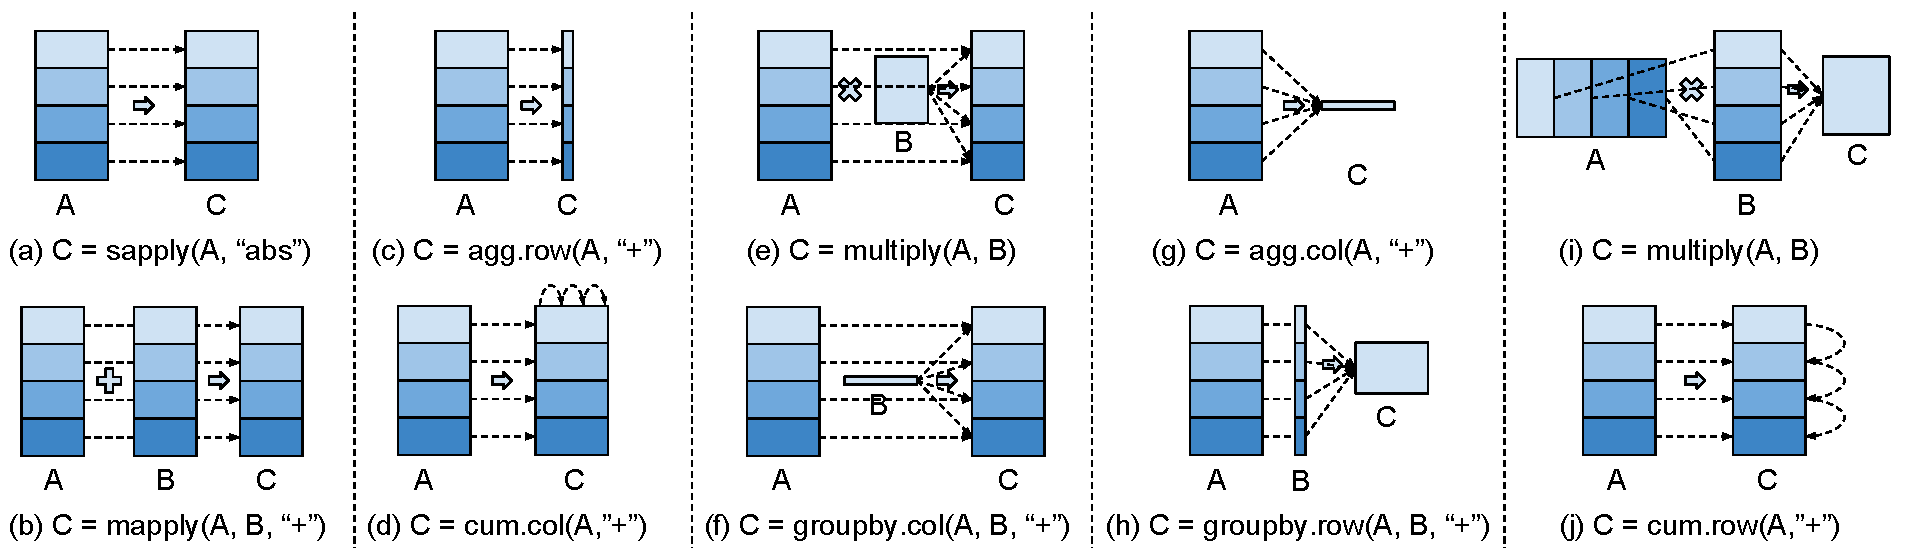
\includegraphics[scale=0.5]{FlashMatrix_figs/Parallelize.pdf}
	\vspace{-4pt}
	\caption{Data flow for the GenOps in Table \ref{tbl:genops} on tall matrices
	 with 1D partitioning.}
	\label{fig:parallel}
  \vspace{-8pt}
\end{figure*}

Parallelization strategies in FlashR vary based on the matrix operations
and matrix shape because matrix operations have various data dependencies
(Figure \ref{fig:parallel}). Currently, FlashR parallelizes matrix operations
with 1D partitioning, because most of machine learning datasets have many more
samples than features.

\begin{itemize}
	\item For operations illustrated in Figure \ref{fig:parallel}
		(a, b, c, d), a partition $i$ of the output matrix solely depends
		on partitions $i$ of the input matrices. This significantly simplifies
		parallelization. Partitions $i$ of all matrices are assigned to
		the same thread to avoid remote memory access. There is no data sharing
		among threads.
	\item For operations in Figure \ref{fig:parallel} (e, f), a partition
		$i$ of the output matrix still solely depends on a partition
		$i$ of the input matrix $A$, but the input matrix
		$B$ is shared by all threads. Because matrix $B$ is
		read-only, threads do not need synchronization to perform computation.
		Matrix $B$ is generally small, so FlashR always keeps it in memory.
	\item For operations in Figure
		\ref{fig:parallel} (g, h, i), the output matrix contains the aggregation
		over all partitions of the input matrices. To parallelize these operations,
		FlashR maintains a local buffer for the partial aggregation result in each
		thread and combines all partial results at the end of
		the computation. The local buffers may grow large in
		\textit{groupby.row} because the size of partial aggregation
		results in each thread is determined by the number of different keys in
		the input data. As such, during computation, \textit{groupby.row} merges
		partial aggregation in a local buffer to a global buffer when the size of
		a local buffer reaches a threshold. 
	\item For cumulative operations on a tall matrix in Figure \ref{fig:parallel}
		(j), a partition $i$ of the output matrix depends on a partition $i$ of
		the input matrix as well as a partition $i-1$ of the output matrix.
		Executing this operation in parallel typically requires two passes over
		the input data \cite{Ladner1980}: the first pass builds a tree of
		aggregation bottom-up and the second pass traverses the tree top-down
		to compute the final result. To reduce I/O and evaluate this operation with
		other operations together (Section \ref{sec:materialize}), FlashR performs
		computation in a cumulative operation with a single scan over input
		data. To perform cumulative operations efficiently in parallel, FlashR
		takes advantage of sequential task dispatching and asynchronous data access.
		FlashR maintains
		a current global accumulated result and a small set of local accumulated
		results from some partitions, and shares them among all threads. If the data
		that a partition $i$ depends on is ready, a thread computes the partition
		and passes it to the subsequent matrix operations. Otherwise, a thread moves
		to the next partition $i+1$ and gets its dependency data ready. If the number
		of pending partitions reaches a threshold, a thread puts itself to sleep
		and waits for all dependency data to become available.
\end{itemize}

%\dz{NUMA optimizations.}
%dispatch computation tasks in a NUMA-aware fashion.

%\dz{Most of computation requires to access partitions of a matrix sequentially.
%This allows us to virtualize some operations that we don't know the size of
%output in advance. e.g., read text input and filter operation.}

%For a block matrix with many TAS matrices, we parallelize the computation and
%I/O access differently. One of the goals is to reduce memory consumption.
%Instead of getting the row/column range from all TAS matrices before performing
%computation, we read the row/column range from some TAS matrices first, perform
%computation and move on to the next TAS matrices in the same range. This is
%very helpful if the computation is aggregation.

\subsection{Lazy evaluation}\label{sec:lazyeval}

In practice, FlashR almost never evaluates a single matrix operation alone.
Instead, it always evaluates matrix operations in Section \ref{sec:api}
lazily and constructs directed acyclic graphs (DAG) to represent computation.
Lazy evaluation is essential to achieve substantial performance for a sequence
of matrix operations in a deep memory hierarchy. FlashR grows each DAG as large
as possible so that later on it evaluates all matrix operations inside a DAG
in a single parallel execution to increase the ratio of computation to I/O.

With lazily evaluation, matrix operations
output \textit{virtual matrices} that represent the computation result,
instead of storing data physically. In the current implementation,
the only operations that are not lazily evaluated are operations that
load data from external sources, such as \textit{load.dense} and
\textit{load.sparse}, and the operations that output matrices
with the size depending on data of the input matrices, such as \textit{unique}
and \textit{table}.
\textit{Virtual matrices} materialize data on the fly during computation
and transfer output as input to the subsequent matrix operation.
A matrix operation on a \textit{block matrix} may output
a block \textit{virtual matrix}.

%\dz{There are two types of virtual matrices. Most of the virtual matrices
%are reporducible (each access returns the same value). The computation in
%the other type of virtual matrices may not be reproduciable and thus, we
%store the computation result once data is generated (e.g., random matrix).}

Some of the matrix operations output matrices with
a different \textit{partition dimension} size than the input matrices and,
in general, forms the edge nodes of a DAG. We denote these matrices as
\textit{sink matrices}. Operations, such as aggregation and groupby,
output \textit{sink matrices}. \textit{Sink matrices} tend to be small and, once
materialized, their materialized results are stored in memory.
%The maximum size of a sink matrix from an aggregation
%is $\sqrt{N}$ for $N$ elements in the input matrix and for groupby
%$k \times \sqrt{N}$ for $k$ groups, where $k$ is usually a small number.
%For most of machine learning and data analysis tasks, the output of inner product
%of a wide matrix with a tall matrix is small because
%the long dimension of these matrices is much larger than the short dimension.

Figure \ref{fig:dag} (a) shows an example of DAG that represents the computation
of the k-means algorithm. A DAG comprises a set of
matrix nodes (rectangles) and computation nodes (ellipses). The majority of
matrix nodes are virtual matrices (dashed line rectangles).
In this example, only the input matrix \textit{X} has materialized data.
A computation node references a GenOp and input matrices and
may contain some immutable computation state, such as scalar variables and
small matrices. 

\subsection{DAG materialization}\label{sec:materialize}
FlashR evaluates all computation in a DAG in a single parallel execution
and fuses matrix operations to reduce data
movement in the memory hierarchy to achieve efficiency. This data-driven,
operation fusion allows out-of-core problems to approach in-memory speed.

FlashR allows both explicit and implicit DAG materialization to simplify
programming while providing the opportunity to tune the code for
better speed. For explicit materialization, a user can invoke the
\textit{materialize} function in Table \ref{tbl:utility} to materialize
a virtual matrix. Implicit materialization includes access to individual
elements of a sink matrix and invoking matrix operations whose output size
depends on input data, such as \textit{unique} and \textit{table}. Materialization
on a virtual matrix triggers materialization on the DAG where the virtual
matrix connects.

By default, FlashR saves the computation results of all sink matrices of
the DAG in memory and discards the data of non-sink matrices on the fly.
Because sink matrices tend to be small, this rule leads to small memory
consumption. In exceptional cases, especially for iterative algorithms,
it is helpful to save some non-sink matrices to avoid
redundant computation and I/O across iterations.  We allow users to
set a flag on any virtual matrix with \textit{set.cache} to materialize and
cache data in memory or on SSDs during computation, similar to caching
a resilient distributed dataset (RDD) in Spark \cite{spark}.
Internally, FlashR uses this mechanism to lazily evaluate \textit{runif.matrix}:
FlashR generates random numbers when the matrix is used for the first time and
the generated random numbers are cached so that the matrix returns the same
data when the matrix is accessed again.

\begin{figure}
	\centering
	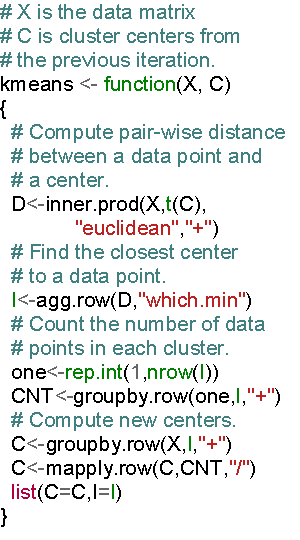
\includegraphics[scale=0.6]{FlashMatrix_figs/kmeans.pdf}
  \vspace{-4pt}
	\caption{(a) Matrix operations are lazily evaluated to form
	a directed-acyclic graph (DAG); (b) The data flow in DAG materialization
	with two levels of partitioning: matrix X on SSDs is first partitioned
	and is read to memory in I/O partitions; an I/O partition is further
	split into processor cache (Pcache) partitions; once a Pcache partition
	is materialized, it is passed to the next GenOp to reduce CPU cache misses. }
	\label{fig:dag}
  \vspace{-8pt}
\end{figure}

FlashR partitions matrices in a DAG and materializes partitions separately in
most cases. This is possible because all matrices in a DAG except sink matrices
share the same \textit{partition dimension} and the same I/O partition size.
As illustrated in Figure \ref{fig:dag} (b), a partition $i$ of a virtual
matrix requires data only from partitions
$i$ of the parent matrices.  All DAG operations in a partition are processed by 
the same thread so that all data required by the computations are stored and
accessed in the memory close to the processor to increase the memory bandwidth
in a NUMA machine.

FlashR uses two-level partitioning on dense matrices to reduce data movement
between SSDs and CPU (Figure \ref{fig:dag} (b)). It reads data on SSDs in
I/O partitions and assigns these partitions to a thread as a parallel task.
It further splits I/O-partitions into processor cache (Pcache) partitions
at runtime.  Each thread materializes one Pcache-partition at a time from
a matrix. Regular tall matrices are divided into TAS matrices and matrix
operations are converted to running on these TAS matrices instead. As such,
a Pcache-partition is sufficiently small to fit in the CPU L1/L2 cache.

To reduce CPU cache pollution and reduce data movement between CPU and memory,
a thread performs depth-first traversal in a DAG and evaluates matrix operations
in the order that they are traversed. Each time, a thread performs a matrix
operation on a Pcache partition of a matrix and passes the Pcache partition to
the subsequent matrix operation, instead of materializing the next Pcache partition.
This ensures that a Pcache partition resides in the CPU cache when the next
matrix operation consumes it. In each thread, all intermediate matrices have
only one Pcache partition materialized at any time.

To further reduce CPU cache pollution, FlashR recycles memory buffers used
by Pcache partitions in the CPU cache. FlashR maintains a counter on each
Pcache partition. When the counter indicates the partition has been used
by all subsequent matrix operations, the memory buffer of the partition is
recycled and used to store the output of
the next matrix operation. As such, the next matrix operation writes
its output data in the memory that is already in CPU cache.

\section{Machine learning algorithms} \label{sec:apps}
To illustrate the programming interface of FlashR, we showcase some classic
algorithms written in FlashR. One is implemented with R \textit{base} functions
and can run in the existing R framework without any modification, and the other
is written with GenOps.

\begin{figure}
\centering
\begin{minted}[mathescape,
	fontsize=\footnotesize,
	frame=single,
	tabsize=2,
	]{R}
# X is the data matrix. C is cluster centers.
kmeans.iter <- function(X,C) {
	# Compute pair-wise distance.
	D<-inner.prod(X,t(C), "euclidean","+")
	# Find the closest center.
	I<-agg.row(D,"which.min")
	# Count the number of data points in each cluster.
	CNT<-groupby.row(rep.int(1,nrow(I)),I,"+")
	# Compute the new centers.
	C<-sweep(groupby.row(X,I,"+"),2,CNT,"/")
	list(C=C,I=I)
}
\end{minted}
\vspace{-10pt}
	\caption{The FlashR implementation for an iteration of k-means.}
	\label{fig:kmeans}
\vspace{-10pt}
\end{figure}

K-means is a commonly used clustering algorithm that partitions data points
into $k$ clusters and minimizes the mean distance between the data points and
the cluster center. We use this algorithm to illustrate programming with GenOps
(Figure \ref{fig:kmeans}). It uses \textit{inner.prod} to
compute the Euclidean distance between every data point and every cluster center
and outputs a matrix with each row representing the distances to centers.  
It uses \textit{agg.row} to find the closest
cluster for each data point.  The output matrix 
assigns data points to clusters. It then uses \textit{groupby.row} to count
the number of data points in each cluster and compute the mean of each cluster.

\begin{figure}
\begin{minted}[mathescape,
fontsize=\footnotesize,
frame=single,
tabsize=2,
]{R}
# `X' is the data matrix, whose rows represent data points.
# `y' stores the labels of data points.
logistic.regression <- function(X,y) {
	grad <- function(X,y,w)
		(t(X)%*%(1/(1+exp(-X%*%t(w)))-y))/length(y)
	cost <- function(X,y,w)
		sum(y*(-X%*%t(w))+log(1+exp(X%*%t(w))))/length(y)
	# Gradient descent with line search.
	theta <- matrix(rep(0, num.features), nrow=1)
	for (i in 1:max.iters) {
		g <- grad(X, y, theta)
		l <- cost(X, y, theta)
		eta <- 1
		delta <- 0.5 * (-g) %*% t(g)
		while (cost(X, y, theta+eta*(-g)) < l+delta*eta)
			eta <- eta * 0.2
		theta <- theta + (-g) * eta
	}
	theta
}
\end{minted}
\vspace{-10pt}
\caption{A simplified implementation of logistic regression using
steepest gradient descent in FlashR.}
\label{logistic}
\vspace{-5pt}
\end{figure}

Logistic regression is a commonly used classification algorithm.
We implement this algorithm solely with the R \textit{base} functions
overridden by FlashR. Figure
\ref{logistic} implements logistic regression for problems with binary-class
labels. It uses steepest gradient descent with line search to minimize
the \textit{cost} function. This example does not have a regularization term
in the cost function.

%PageRank is a well-known algorithm for graph analysis. The matrix formulation
%(Figure \ref{pagerank}) operates on the adjacency matrix of a graph. It uses
%a power method and performs a sequence of sparse matrix multiplications until
%the algorithm converges.
%\begin{figure}
%\begin{minted}[mathescape,
%fontsize=\footnotesize,
%frame=single,
%tabsize=2,
%]{R}
%# `graph' is a sparse matrix that represents
%# the input graph. `d' is a damping factor,
%# `epsilon' is the convergence accuracy.
%pagerank<-function(graph,d=0.15,epsilon=1e-2){
%	N <- nrow(graph)
%	pr1 <- fm.rep.int(1/N, N)
%	out.deg <- graph %*% fm.rep.int(1, N)
%	converge <- 0
%	graph <- t(graph)
%	while (converge < N) {
%		pr2 <- (1-d)/N+d*(graph %*% (pr1/out.deg))
%		diff <- abs(pr1-pr2)
%		converge <- sum(diff < epsilon)
%		pr1 <- pr2
%	}
%	pr1
%}
%\end{minted}
%\vspace{-10pt}
%\caption{A simplified implementation of PageRank in FlashR.}
%\label{pagerank}
%\vspace{-10pt}
%\end{figure}
